\documentclass{beamer}
%\documentclass[handout]{beamer}

%\includeonlyframes{bsm,title,toc,imprint-mouse-devel,igf2-imprint-evol,sister-disorders,previous-age-studies,our-study,cmc,toc-current,filtering-calling,fitting-models,ll-surface,all-betas,orthogonality,identifiability,anova,betas-cluster,signif-genes,cf-overall-expression,summary,improving-model,p-val,imprinted-brain,chess-lab}

% language settings
%\usepackage{fontspec, polyglossia}
%\setdefaultlanguage{magyar}

% common packages
\usepackage{amsmath, multimedia, hyperref, color, multirow}
%\usepackage{graphicx}

% TikZ
\usepackage{tikz}
%\usetikzlibrary{arrows.meta, decorations.pathmorphing, decorations.pathreplacing, shapes.geometric,mindmap}
%\usetikzlibrary{shapes.geometric,fadings,bayesnet}

% beamer styles
\mode<presentation>{
%\usetheme{Pittsburgh}
\usetheme{Copenhagen}
\usecolortheme{beaver}
%\usecolortheme{seahorse}
%\usefonttheme{structureitalicserif}
\setbeamercovered{transparent}
}
\setbeamertemplate{blocks}[rounded][shadow=true]
\AtBeginSubsection[]{
  \begin{frame}<beamer>{Contents}
    %\tableofcontents[currentsection]
    \tableofcontents[currentsubsection]
  \end{frame}
}
%\useoutertheme[]{tree}

\title{Genomic Imprinting in the Human Brain}
\author{Attila Guly\'{a}s-Kov\'{a}cs}
\date{Chess Lab}

\newcommand{\platefigscale}[0]{0.7}
\newcommand{\ownfigscale}[0]{0.4}

\begin{document}

\begin{frame}[plain, label=title]
\maketitle
\end{frame}

\begin{frame}{Contents}
\tableofcontents
\end{frame}

\section{First part}

\subsection{Imprinting and allelic bias}

\begin{frame}{Imprinting and allelic bias}
\begin{enumerate}
\item epigenetic mechanism
\item variation across time and tissue
\item biological function 
\end{enumerate}
\includegraphics[width=0.6\textwidth]{figures/from-others/renfree-2012-fig2.jpg}

{\tiny Renfree et al 2012 Philos Trans R Soc Lond B}

\end{frame}

\begin{frame}{Increasing evolutionary prevalence}{}
How many imprinted genes?

\(\approx 100 \; \leftrightarrow \; \approx 1300\) \footnote{Gregg et al 2010}

\includegraphics[width=0.7\textwidth]{figures/from-others/smits-et-al-2008-fig5.jpg}

{\tiny Smits et al 2008 Nat Genet}
\end{frame}

% shift away from normal allelic bias in two possible directions => sister disorders
% general: growth disorders, mental defects
% Igf2/H19: Beckwith–Wiedeman syn, Silver-Russell syn
% Ube3a cluster 15q13: Angelman (mental retardation); Prader-Willi (obesity, mental defects)
% CNV in 15q13 increases risk of SCZ, a highly polygenic disorder with many common variants with mild risk
\begin{frame}[t, label=sister-disorders]{Dysfunction: development and growth}
\includegraphics[width=0.85\textwidth]{figures/from-others/peters-2014-imprinting-fig1b.jpg}
{\tiny Peters 2014}
\begin{columns}[t]
\begin{column}{0.5\textwidth}
{\footnotesize Angelman syndrome}

\includegraphics<1>[width=0.60\columnwidth]{figures/from-others/boy-with-a-puppet-Giovanni-Francesco-Caroto.jpg}

{\tiny Boy with a Puppet}
\end{column}
\begin{column}{0.5\textwidth}
{\footnotesize Prader-Willi syndrome}

\includegraphics<1>[width=0.60\columnwidth]{figures/from-others/Eugenia-Martínez-Vallejo-clothed-cropped.jpg}

{\tiny Eugenia Mart\'{i}nez Vallejo}
\end{column}
\end{columns}

\end{frame}

\begin{frame}{Dysfunction: psychiatry}{Angelman/Prader-Willi region implicated
in schizophrenia}
\includegraphics[width=1.0\textwidth]{figures/from-others/sullivan-natrevgenet-2012-fig1b.jpg}

{\tiny Sullivan 2012 Nat Rev Genet.}
\end{frame}

%% uses kinship theory to explain psychiatric conditions
%% PEGs self-oriented cognition, - inc. fitness, autistic; MEGs mentalistic cognition, + incl. fitness, psychotic
%% this hypothesis guides the study the role of imprinting in psychiatric disorders e.g. SCZ
%\begin{frame}[label=imprinted-brain]{The imprinted brain theory}
%\begin{center}
%\includegraphics[width=0.7\textwidth]{figures/from-others/crespi-2008-fig3.png}
%\vfill
%{\tiny \raggedright{Crespi \& Badcock 2008 Behav Brain Sci.}}
%\end{center}
%\end{frame}

%% clarifying the functional roles of imprinted genes requires characterization of their variation
%% variation across devel. time, tissue type, gender,...
%% variation in postnatal age, aging unclear especially in humans
%% theoretical and experimental mouse studies
%\begin{frame}[label=previous-age-studies]{Variation with age}
%\begin{columns}[t]
%\begin{column}{0.5\textwidth}
%
%\includegraphics[height=0.5\textheight]{figures/from-others/ubeda-2012-fig3a.jpg}
%
%{\tiny Ubeda 2012 Evolution}
%\end{column}
%
%\begin{column}{0.5\textwidth}
%
%\includegraphics[height=0.3\textheight]{figures/from-others/perez-2015-elife-fig4b.png}
%
%{\tiny Perez et al 2015 eLife}
%\end{column}
%\end{columns}
%\end{frame}

\begin{frame}<1>[label=questions]{\textit{Questions} \only<2->{and \textbf{Answers}}}
\begin{enumerate}
\item Imprinted genes in the DLPFC\footnote{dorsolateral prefrontal
cortex}
\begin{itemize}
\item \textit{How many?} \only<2->{\textbf{30 genes in \(\approx\frac{1}{3}\) genome}}
\item \textit{Novelty?} \only<2->{\textbf{8 new imprinted genes}}
\end{itemize}
\item Dependence of allelic bias...\\on age, psychiatric condition, genetics
(ancestry),
gender
\begin{itemize}
\item \textit{Signal vs noise?} \only<3>{\textbf{Poor; modeling challenge}}
\item \textit{Genes affected uniformly?} \only<3>{\textbf{No}}
\item \textit{Most prominent effects?} \only<3>{\textbf{genetics and age on a few genes}}
\end{itemize}
\end{enumerate}
\end{frame}

\subsection{Imprinted genes in the DLPFC}

\begin{frame}{The read count ratio approach}

\includegraphics[width=1.0\textwidth]{figures/from-others/castel-2015-fig1.png}

{\tiny Castel et al 2015 GenomeBiology}
\end{frame}

% our study aims to characterize that variation in humans using CMC data
\begin{frame}[label=our-study]{Our research study}
\begin{description}
\item[data/project] Common Mind Consortium
\item[participants] \alert{Ifat Keydar}, Eva Xia, Menachem Fromer, Doug Ruderfer, Ravi Sachinanandam, Andrew Chess
\end{description}
\end{frame}

% observational study: explain the observed variation in allelic bias with variation in age, gender, psych. condition
% e.g. gene g1 has stronger maternal bias in individual i1 than in i2
% allelic bias not directly observed; RNA-seq read count ration S statistic; technical noise
\begin{frame}[label=cmc]{Study setup}
% CommonMind: within cohort variation of age, gender, genotype, Dx; correlate
% with RNA-seq-based measure of allelic bias
\includegraphics[height=0.75\textheight]{figures/by-me/commonmind-rna-seq/commonmind-rna-seq.pdf}
\end{frame}

\begin{frame}[t]{Distribution across individuals and genes}
\begin{center}
\includegraphics[height=0.8\textheight]{figures/2016-07-19-genome-wide-S/complex-plot-b-1.png}
\end{center}
\end{frame}

% based on read count and S we filtered genes and called imprinted genes
% we used the eCDF of S (shades of color) as well as a simple test for biallelic expr (black)
% 30 genes called imprinted, most previously known, few novel
\begin{frame}[label=filtering-calling]{Called imprinted genes}
%{Consistent with \(\approx100\) imprinted genes genome-wide}
\begin{columns}[t]
\begin{column}{0.4\textwidth}

\includegraphics[height=0.85\textheight]{figures/2016-08-01-ifats-filters/top-ranking-genes-2.pdf}
\end{column}

\begin{column}{0.6\textwidth}

\includegraphics[height=0.8\textheight]{figures/2016-08-01-ifats-filters/venn-total-finalf-called-1.pdf}
\end{column}
\end{columns}
\end{frame}

\againframe<2>{questions}

\section{Second part}

\subsection{Dependence of allelic bias}

\begin{frame}{Explaining inter-individual variation}
\begin{columns}[t]
\begin{column}{0.4\textwidth}

\includegraphics[width=1.1\columnwidth]{figures/2016-07-19-genome-wide-S/complex-plot-1.png}
\end{column}

\begin{column}{0.6\textwidth}

\includegraphics[width=1.1\columnwidth]{figures/2016-06-26-trellis-display-of-data/S-age-gender-2}
\end{column}
\end{columns}
\end{frame}

\begin{frame}{Multiple interdependent predictors}
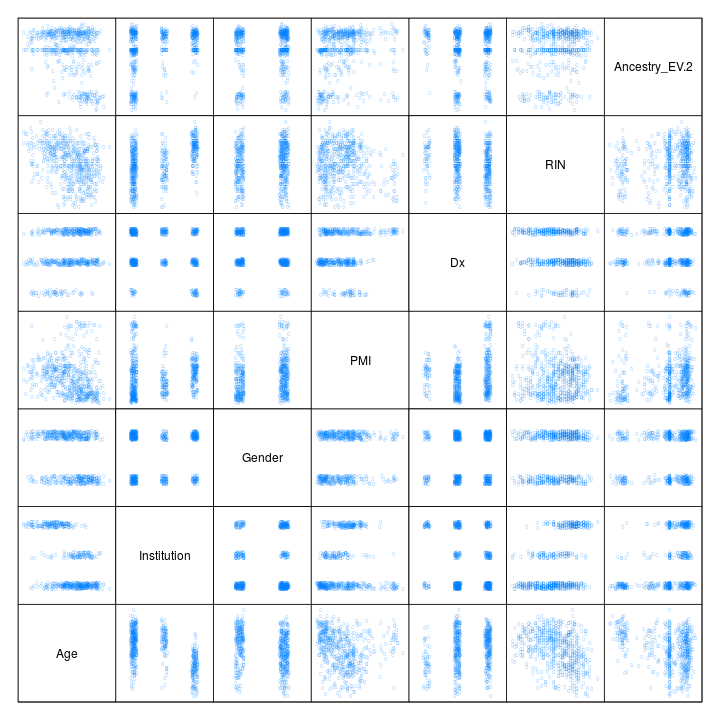
\includegraphics[width=0.9\textheight]{figures/2016-06-26-trellis-display-of-data/evar-scatterplot-matrix-1.png}
\end{frame}

\begin{frame}[t]{Inferring dependence using regression models}
\begin{columns}[t]
\begin{column}{0.4\textwidth}

generalized linear models

\begin{eqnarray*}
\mathrm{E}[y_g] &=& \mu_g = h^{-1}(X\beta_g) \\
y &=& \mu_g + \varepsilon_{\mu_g}
\end{eqnarray*}
\end{column}

\begin{column}{0.6\textwidth}

\visible<2->{inference for gene \(g\) (PEG3)}

%\includegraphics<2>[width=1.1\columnwidth]{figures/2016-08-21-likelihood-surface/explain-rll-wireframe-1.png}
\includegraphics<2>[width=\columnwidth]{figures/2016-08-21-likelihood-surface/explain-rll-levelplot-B-1.png}
\end{column}
\end{columns}

\end{frame}

\begin{frame}[t]{Selection among several models}
\begin{columns}[t]
\begin{column}{0.5\textwidth}
predictive distributions

\tiny{(simple regression, for demonstration only)}

\includegraphics[width=1.1\columnwidth]{figures/2016-08-23-glm-sampling-distributions/PEG3-1.png}
\end{column}

\begin{column}{0.5\textwidth}
\only<2>{result:
\vfill
AIC isn't useful in this case\\
\tiny{bad fit may inflate likelihood for some models}}
\only<3>{normality of residuals}
\only<4>{homogeneity of error}
\only<5>{influence of outliers}
\only<6>{result:
\vfill
wnlm.Q and unlm.Q fit the best}

\only<3-5>{\tiny{(multiple regression)}}

\includegraphics<3>[width=1.1\columnwidth]{figures/2016-09-23-model-checking/qqnorm-PEG3-1.png}
\includegraphics<4>[width=1.1\columnwidth]{figures/2016-09-23-model-checking/homoscedas-PEG3-1.png}
\includegraphics<5>[width=1.1\columnwidth]{figures/2016-09-23-model-checking/influence-PEG3-1.png}
\end{column}
\end{columns}
\end{frame}

\begin{frame}{Explained variation of read count ratio}

\includegraphics[width=0.9\textwidth]{figures/2017-02-14-beta-from-mixed-model/tval-varpart-fixed-present-1.pdf}
\end{frame}

\begin{frame}[label=signif-genes]{Genes \(g\) affected by one or more predictors \(p\)
(\(\beta_{pg}\neq 0\))}
%{Test: parametric + non-parametric (permutations)}
\tiny
\begin{tabular}{lllll}
Gene & Gene type & Chr & Coefficient & Known phenotype\\
\hline
ZDBF2 & protein coding & 2 & Age,  Ancestry.1 & \\
NAP1L5 & protein coding & 4 & GenderMale & \\
PEG10 & protein coding & 7 & DxSCZ & \\
MEST & protein coding & 7 & DxSCZ & Silver-Russell syndrome\\
KCNK9 & protein coding & 8 & Age & Birk-Barel mental retardation dysmorphism syndrome\\
INPP5F & protein coding & 10 & Age & cell motility; endocytic recycling\\
KCNQ1OT1 & antisense & 11 & GenderMale & Beckwith-Wiedemann syn.; Isol.~hemihyperplasia\\
MEG3 & lincRNA & 14 & GenderMale & Mat/pat 14q32.2 hypermeth/microdel syndrome\\
RP11-909M7.3 & lincRNA & 14 & DxSCZ & \\
AL132709.5 & miRNA & 14 & Ancestry.1 & \\
MAGEL2 & protein coding & 15 & Age & Prader-Willi syn.; Schaaf-Yang syn.;
Arthrogryposis \\
NDN & protein coding & 15 & GenderMale & Prader-Willi syndrome\\
PWRN1 & lincRNA & 15 & Ancestry.1 & Prader-Willi syndrome\\
UBE3A & protein coding & 15 & DxSCZ & Prader-Willi syn.; Angelman syn.; circadian rhythm\\
PEG3 & protein coding & 19 & GenderMale & \\
\end{tabular}

\end{frame}

\begin{frame}{Different results under similarly well-fitting models}

\includegraphics[height=0.85\textheight]{figures/2016-06-22-extending-anova/unlm-Q-wnlm-Q-compare-1.pdf}
\end{frame}

% two predictors interact when the effect of one predictor (X1) depends on the value (a or b) of another (X2) 
% this is distinct from correlation/non-orthogonality of predictors
% e.g. if X2=a then X1 has no dependence on Y (beta1=0) but if X2=b then it does % (beta1>0)
% we found that effect of Age on S depended on both Institution and Gender at various degrees for different genes
% we didn't model interactions to avoid extra parameters and decrease in power => our conclusions on beta are too simplistic
\begin{frame}[label=interaction]{Effects appear interdependent}
%{The effect of one predictor depends on another}

\includegraphics[width=0.9\textwidth]{figures/2016-07-08-conditional-inference/beta-age-cond-wnlm-Q-2-present-1.pdf}
\end{frame}

\begin{frame}{Multiple levels of variation}
\begin{center}
\includegraphics[height=0.75\textheight]{figures/by-me/commonmind-rna-seq/commonmind-rna-seq.pdf}
\end{center}
\end{frame}

\begin{frame}{Better modeling framework?}
\begin{columns}[t]
\begin{column}{0.5\textwidth}
\begin{center}
regression

\includegraphics[scale=\platefigscale]{figures/by-me/monoall-dependencies-2/obs-simple-general/obs-simple-general.pdf}
\end{center}
\end{column}

\begin{column}{0.5\textwidth}
\begin{center}
hierarchical Bayesian

\includegraphics[scale=\platefigscale]{figures/by-me/monoall-dependencies-2/obs-bayesian/obs-bayesian.pdf}
\end{center}
\end{column}
\end{columns}
\end{frame}

\againframe<3>{questions}

\subsection{Future work}

\begin{frame}{Reanalyze dependence?}
Is it worth? If yes...
\begin{enumerate}
\item add more data
\begin{itemize}
\visible<2>{\item no solution for biased stats.~approach}
\end{itemize}
\item more accurate read counts
\begin{itemize}
\visible<2>{\item improve QC: RNA-seq + genotyping}
\end{itemize}
\item find better model
\begin{itemize}
\visible<2>{\item implement inference, validate}
\end{itemize}
\end{enumerate}
\end{frame}

\begin{frame}{Brain Somatic Mosaicism}
\begin{columns}[t]
\begin{column}{0.6\textwidth}

\includegraphics[width=1.0\columnwidth]{figures/from-others/gage-curropsysbio-2016-1.jpg}

{\tiny Paquola, Erwin, Gage 2016}
\end{column}

\begin{column}{0.4\textwidth}
challenges with somatic variants:
\begin{itemize}
\item detection\\
{\footnotesize allelic fraction}
\item prioritization\\{\footnotesize multiple info}
\item integration\\{\footnotesize germline vars.}
\end{itemize}
\end{column}
\end{columns}
\end{frame}

\begin{frame}[label=chess-lab]{Thanks to}
\begin{columns}[t]
\begin{column}{0.5\textwidth}

Chess lab
\begin{itemize}
\item Andy Chess {\footnotesize (support)}
\item Chaggai Rosenbluh {\footnotesize (feedback)}
\item Eva Xia
\item Mehaa Bajaj   
\end{itemize}

\includegraphics[width=0.6\columnwidth]{figures/from-others/chess-board.jpg}
\end{column}

\begin{column}{0.5\textwidth}
\begin{itemize}
\item Gabriel Hoffman\\
{\footnotesize (feedback, variancePartition)}
\item Ravi Sachinanandam\\
{\footnotesize (critical feedback)}
\end{itemize}
\end{column}
\end{columns}
\end{frame}

\end{document}


\begin{columns}[t]
\begin{column}{0.5\textwidth}

\end{column}

\begin{column}{0.5\textwidth}

\end{column}
\end{columns}

% 1% of genes are imprinted in mice
% imprints are sex-specific methylated DNA regions generated in gametogenesis
% this results in allelic bias in the expression of imprinted genes in the progeny
% complete bias: monoallelic expression
\begin{frame}[label=imprint-mouse-devel]{Genomic imprints during development}
\begin{center}
\includegraphics[height=0.7\textheight]{figures/from-others/plasschaert-bartolomei-2014-fig1.jpeg}
\vfill
{\tiny Plasschaert \& Bartolomei 2014 Development.}
\end{center}
\end{frame}

% Igf2 and H19: among the first genes found imprinted in mice
% methylation imprint inhibits both the insulator for Igf2 and the promoter for H19
% embryonic/placental growth: paternally expressed Igf2 promotes, mat. exp. H19 inhibits it
% most imprinted genes play role in placental development and expressed in embryo/placenta
% further roles: postnatal growth, maternal behavior, metabolism, REM sleep
% this fits co-occurrence of placentation and evol. of imprinting
% kinship theory of imprinting: interactions (e.g. among siblings), inclusive fitness, relatedness
% maternal half siblings: closer relatedness of maternal genes than paternal genes => conflict
% resolution: growth promoting genes paternally biased, growth inhibiting maternally (e.g. Igf2, H19)
\begin{frame}[label=igf2-imprint-evol]{Allelic bias and placental development}{}
\begin{columns}[t]
\begin{column}{0.4\textwidth}

\includegraphics[width=\columnwidth]{figures/from-others/renfree-2012-fig2.jpg}

{\tiny Renfree et al 2012 Philos Trans R Soc Lond B}

\end{column}

\begin{column}{0.6\textwidth}

\includegraphics[width=\columnwidth]{figures/from-others/smits-et-al-2008-fig5.jpg}

{\tiny Smits et al 2008 Nat Genet}
\end{column}
\end{columns}
\begin{center}
\end{center}
\end{frame}

\begin{frame}[label=kinship-theory]{Kinship theory}
{Application of kin selection to imprinting}
\begin{center}
\begin{columns}[t]
\begin{column}{0.5\textwidth}

\includegraphics[width=0.8\columnwidth]{figures/from-others/nowak-et-al-2010-fig1top.jpg}
\end{column}

\begin{column}{0.5\textwidth}

\includegraphics[width=0.7\columnwidth]{figures/from-others/nowak-et-al-2010-fig3ab.jpg}
\end{column}
\end{columns}
{\tiny Nowak et al 2010 Nature}
\end{center}
\end{frame}

% shift away from normal allelic bias in two possible directions => sister disorders
% general: growth disorders, mental defects
% Igf2/H19: Beckwith–Wiedeman syn, Silver-Russell syn
% Ube3a cluster 15q13: Angelman (mental retardation); Prader-Willi (obesity, mental defects)
% CNV in 15q13 increases risk of SCZ, a highly polygenic disorder with many common variants with mild risk
\begin{frame}[t, label=sister-disorders]{Sister disorders, neuropsychiatric functions}
\includegraphics[width=0.65\textwidth]{figures/from-others/peters-2014-imprinting-fig1b.jpg}
{\tiny Peters 2014 Nat Rev Genet.}
\visible<1>{
\begin{columns}[t]
\begin{column}{0.5\textwidth}
{\footnotesize Angelman syndrome}

\includegraphics<1>[width=0.65\columnwidth]{figures/from-others/boy-with-a-puppet-Giovanni-Francesco-Caroto.jpg}

{\tiny Boy with a Puppet}
\end{column}
\begin{column}{0.5\textwidth}
{\footnotesize Prader-Willi syndrome}

\includegraphics<1>[width=0.65\columnwidth]{figures/from-others/Eugenia-Martínez-Vallejo-clothed-cropped.jpg}

{\tiny Eugenia Mart\'{i}nez Vallejo}
\end{column}
\end{columns}
}

\visible<2>{
\footnotesize genetic architecture of schizophrenia
\includegraphics[width=0.7\textwidth]{figures/from-others/sullivan-natrevgenet-2012-fig1b.jpg}
{\tiny Sullivan 2012 Nat Rev Genet.}
}
\end{frame}

% uses kinship theory to explain psychiatric conditions
% PEGs self-oriented cognition, - inc. fitness, autistic; MEGs mentalistic cognition, + incl. fitness, psychotic
% this hypothesis guides the study the role of imprinting in psychiatric disorders e.g. SCZ
\begin{frame}[label=imprinted-brain]{The imprinted brain theory}
\begin{center}
\includegraphics[width=0.7\textwidth]{figures/from-others/crespi-2008-fig3.png}
\vfill
{\tiny \raggedright{Crespi \& Badcock 2008 Behav Brain Sci.}}
\end{center}
\end{frame}

\subsection{Our study: motivation \& design}

% clarifying the functional roles of imprinted genes requires characterization of their variation
% variation across devel. time, tissue type, gender,...
% variation in postnatal age, aging unclear especially in humans
% theoretical and experimental mouse studies
\begin{frame}[label=previous-age-studies]{Explaining variation of allelic bias: age}
\begin{columns}[t]
\begin{column}{0.5\textwidth}

\includegraphics[height=0.5\textheight]{figures/from-others/ubeda-2012-fig3a.jpg}

{\tiny Ubeda 2012 Evolution}
\end{column}

\begin{column}{0.5\textwidth}

\includegraphics[height=0.3\textheight]{figures/from-others/perez-2015-elife-fig4b.png}

{\tiny Perez et al 2015 eLife}
\end{column}
\end{columns}
\end{frame}

% our study aims to characterize that variation in humans using CMC data
\begin{frame}[label=our-study]{Our research study}
\begin{description}
\item[data/project] Common Mind Consortium
%\item[approach] human genomics
\item[questions] imprinted genes in the human brain
\begin{itemize}
\item variation of allelic bias across genes and individuals
\item regulators: age, gender, genotype (ancestry)
\item psychiatric disorders (SCZ, AFF)  
\end{itemize}
\item[participants] \alert{Ifat Keydar}, Eva Xia, Menachem Fromer, Doug Ruderfer, Ravi Sachinanandam, Andrew Chess
\end{description}
\end{frame}

% observational study: explain the observed variation in allelic bias with variation in age, gender, psych. condition
% e.g. gene g1 has stronger maternal bias in individual i1 than in i2
% allelic bias not directly observed; RNA-seq read count ration S statistic; technical noise
\begin{frame}[label=cmc]{The Common Mind data}
% CommonMind: within cohort variation of age, gender, genotype, Dx; correlate
% with RNA-seq-based measure of allelic bias
\includegraphics[height=0.75\textheight]{figures/by-me/commonmind-rna-seq/commonmind-rna-seq.pdf}
\end{frame}

% SEC: Results
\section{Results \& Discussion}
\subsection{Predictors of allelic bias}

\begin{frame}[label=toc-current]
\tableofcontents[currentsection]
\end{frame}

% based on read count and S we filtered genes and called imprinted genes
% we used the eCDF of S (shades of color) as well as a simple test for biallelic expr (black)
% 30 genes called imprinted, most previously known, few novel
\begin{frame}[label=filtering-calling]{Calling imprinted genes}
\begin{columns}[t]
\begin{column}{0.5\textwidth}

\includegraphics[height=0.7\textheight]{figures/2016-08-01-ifats-filters/venn-total-finalf-called-1.pdf}
\end{column}

\begin{column}{0.5\textwidth}

\includegraphics[height=0.7\textheight]{figures/2016-08-01-ifats-filters/top-ranking-genes-1.pdf}
\end{column}
\end{columns}
\end{frame}

% main question: explain variation of allelic bias gaged with read count ratio S
% Y axis: S or Q, a transformed S; X axis: age of death
% green dots: data on PEG3 gene: observations from hundreds of individuals
% phenomenological approach: fit several regression models to data and use the best fitting one(s)
% response Y depending on (explained by) predictor X and reg. coef beta
% predicted curve (black); the slope given by beta; no dependence => beta=0
% noise eps: stochastic variation about the predicted curve, which is not explained by X
% fitting: subjectively, "by eye": compare green cloud to density; objectively: least squares (ML)
% estimate of beta far from 0 and estimation error small => reject H0: beta=0 confidently
% confidence quantified with CIs and p-values
% complication: besides age many other predictors; multiple regression: X based on all of them
\begin{frame}[label=fitting-models]{Explaining variation of allelic bias with predictors}
\begin{columns}[t]
\begin{column}{0.60\textwidth}

\includegraphics<1>[width=\columnwidth]{figures/2016-08-23-glm-sampling-distributions/PEG3-data-only-1.png}
\includegraphics<2->[width=\columnwidth]{figures/2016-08-23-glm-sampling-distributions/PEG3-1.png}

\end{column}

\begin{column}{0.45\textwidth}

\footnotesize
\begin{itemize}
\item \(Y_g\) from read count ratio
\item \(X\) based on predictor(s)
\item \(\mathcal{H}_0:\) no dependence \only<2->{ \(\Leftrightarrow \beta_g = 0 \)}
\end{itemize}
\vfill
\only<2->{
\begin{equation*}
Y_g = X \beta_g + \epsilon_g
\end{equation*}
}
%\begin{tabular}{|r|l|}
%\hline
%response \(Y_g\) & transformation \\
%\hline
%read count ratio \(S_g\) & none \\
%\(Q_g\) & quasi-log \\
%\(R_g\) & rank \\
%\hline
%\end{tabular}

\only<3->{
\tiny
\vfill
\begin{tabular}{|r|l|}
\hline
predictor & levels \\
\hline
Age & \\
Gender & Female, Male\\
Dx & AFF, Control, SCZ\\
Ancestry.1-5 & \\
Institution & MSSM, Penn, Pitt\\
PMI & \\
RIN & \\
RNA\_batch & 0, A, B, C, D, E, F, G, H\\
\hline
\end{tabular}
}
%\includegraphics[scale=\platefigscale]{figures/by-me/monoall-dependencies-2/designed/designed.pdf}

\end{column}
\end{columns}
\end{frame}

\begin{frame}[label=ll-surface]{Estimating \(\beta\) and testing for \(\mathcal{H}_0:\;\beta=0\)}
\begin{columns}[t]
\begin{column}{0.5\textwidth}

\includegraphics[scale=\ownfigscale]{figures/2016-08-21-likelihood-surface/explain-rll-wireframe-1.png}
\end{column}

\begin{column}{0.5\textwidth}

\includegraphics[scale=\ownfigscale]{figures/2016-08-21-likelihood-surface/explain-rll-levelplot-B-1.png}
\end{column}
\end{columns}
\end{frame}

% ML fitting result: wmlm.Q fitted well for all genes and logi.S also fitted well for some genes
% Y axes lists imprinted genes; each panel corresponds to a predictor
% X axes: the H0: beta=0 (red), estimated betas + 99% CIs are shown
% before biol inference I discuss statistical properties that hinder/complicate that inference
\begin{frame}[plain, label=all-betas]
\begin{columns}[t]
\begin{column}{0.5\textwidth}

\includegraphics[height=\textheight]{figures/2016-06-22-extending-anova/reg-coef-wnlm-Q-1.pdf}
\end{column}

\begin{column}{0.5\textwidth}

\includegraphics[height=\textheight]{figures/2016-06-22-extending-anova/reg-coef-logi-S-filt-1.pdf}
\end{column}
\end{columns}
\end{frame}

% contrast designed experiment (mouse) vs observational study (human, CommonMind)
% IN BOTH CASES we have a response Y which either depends on somehow (arrows) or indep of 3 predictors (X_j)
% 3 corresponding betas describe these (in)dependencies; e.g beta2=0
% our data consist of observations on Y and X_j
% A CRUCIAL DIFFERENCE is in the orthogonality of x_.j, the columns of the design matrix
% in designed experiments we determine X_j so we can make them orthogonal
% geometric meaning: equal number (=1) of observations fall on each of the 8 verteces of a cube
% in obs studies we can only observe but not control X_j, which vary randomly and may correlate with each other
% correlations come from either direct dependence between X_j or indirect dependence mediated by e.g. Y
% either way: the result is non-orthognality; the cube becomes slanted, a parallelepiped
% example for X2 -> X3 dependency...
\begin{frame}[t, plain, label=orthogonality]
\begin{columns}[t]
\begin{column}{0.5\textwidth}
designed experiment

\includegraphics[scale=\platefigscale]{figures/by-me/monoall-dependencies-2/designed/designed.pdf}

\end{column}

\begin{column}{0.5\textwidth}
observational study
\includegraphics[scale=\platefigscale]{figures/by-me/monoall-dependencies-2/obs/obs.pdf}
\end{column}
\end{columns}
\vfill

\begin{columns}[t]
\begin{column}{0.5\textwidth}
%orthogonal

\includegraphics[height=0.35\textheight]{figures/from-others/tony-smith-die.png}
\end{column}

\begin{column}{0.5\textwidth}
%non-orthogonal

\includegraphics[height=0.35\textheight]{figures/from-others/tony-smith-new-piece.png}
\end{column}
\end{columns}
\end{frame}

% ...in the CMC data we see that age depends on another predictor, institution
\againframe{cmc}

% non-orthogonality => difficult to differentiate between different submodels using the likelihood based on data
% log-likelihood is a function on multidim param space of several betas => difficult to visualize
% here only 2D slices of LL given by pairs of betas
% the contours of LL are quasi-ellipses delimiting equally likely submodels identified by (beta1, beta2)
% the peak of the LL surface is at the ML estimate of beta
% the ML estmate of beta_Age < 0, beta_RIN => allelic bias decreases with Age and increases with RIN
% within the second contour line the (beta_Age, beta_RIN) are still quite likely
% but non-orthogonality of Age and RIN results in interdependence of likely values of beta_Age and beta_RIN
% so if beta_RIN=0.11 (quite likely), then the most likely value of beta_Age=0 => our conclusion changes on the age effect
\begin{frame}[label=identifiability]{Consequence: poor identifiability}
%{The likelihood of one parameter is linked to another}
\begin{center}
\includegraphics[scale=\ownfigscale]{figures/2016-08-21-likelihood-surface/ll-surf-coefs-wnlm-Q-1.png}
\end{center}
\end{frame}

% non-orthogonality => ANOVA fails
% we cannot estimate the component of variability due to each predictor in isolation from others
\begin{frame}[label=anova]{Consequence: ANOVA is inconclusive}
\begin{center}
\includegraphics[scale=\ownfigscale]{figures/2016-06-22-extending-anova/anova-fw-rv-wnlm-Q-1.pdf}
\end{center}
\end{frame}

% two predictors interact when the effect of one predictor (X1) depends on the value (a or b) of another (X2) 
% this is distinct from correlation/non-orthogonality of predictors
% e.g. if X2=a then X1 has no dependence on Y (beta1=0) but if X2=b then it does % (beta1>0)
% we found that effect of Age on S depended on both Institution and Gender at various degrees for different genes
% we didn't model interactions to avoid extra parameters and decrease in power => our conclusions on beta are too simplistic
\begin{frame}[label=interaction]{Further complication: interaction}
{The effect of one predictor depends on another}
\begin{columns}[t]
\begin{column}{0.4\textwidth}

\includegraphics[scale=\platefigscale]{figures/by-me/monoall-dependencies-2/obs-contextual/obs-contextual.pdf}
\end{column}

\begin{column}{0.6\textwidth}

\includegraphics[width=\columnwidth]{figures/2016-07-08-conditional-inference/beta-age-cond-wnlm-Q-2-1.pdf}
\end{column}
\end{columns}
\end{frame}

\againframe[plain]{all-betas}

% Age, Gender, psych. condition (Dx) and genetics (Ancestry.1) all effect one gene or another
% all 4 predictors, in particular Age, may both increase or decrease allelic bias
% SCZ is associated to allelic bias of several genes consistent with imprinted brain theory
% there seems to be some variability within imprinted gene clusters suggesting they are not regulated exclusively in a concerted fashion
% comparing these results to those under the log.S model shows reasonable agreement
\begin{frame}[label=betas-cluster]
{The main results}
\begin{columns}[t]
\begin{column}{0.5\textwidth}
\begin{center}
biological effects

\includegraphics[width=\columnwidth]{figures/2016-08-08-imprinted-gene-clusters/segplot-wnlm-Q-99conf-1.pdf}

\tiny
model: wnlm.Q
\end{center}
\end{column}

\begin{column}{0.5\textwidth}
\begin{center}
\only<2->{agreement between models}

\includegraphics<2->[width=\columnwidth]{figures/2016-06-22-extending-anova/logi-S-filtered-wnlm-Q-compare-4pred-1.pdf}
\end{center}
\end{column}
\end{columns}
\end{frame}

% p-values for the H0: beta=0 calculated in 2x2 methods
% method 1 vs 2 (wnlm.Q) and 3 vs 4 (logi.S): parametric vs non-parametric
% the agreement is good but not perfect => difficulty of making inferences based on multiple plausible models
% heuristic rule: method 1 AND method 2; ignore methods 3,4 because Andy doesn't like logi.S
\begin{frame}[label=p-val]{p-values for \(\mathcal{H}_0:\) no dependence}
\begin{center}
\includegraphics[scale=\ownfigscale]{figures/2016-10-03-permutation-test/p-values-1.pdf}
\end{center}
\end{frame}

\begin{frame}[label=signif-genes]{Affected genes (\(\mathcal{H}_0\) rejected)}
%{Test: parametric + non-parametric (permutations)}
\tiny
\begin{tabular}{lllll}
Gene & Gene type & Chr & Coefficient & Known phenotype\\
\hline
ZDBF2 & protein coding & 2 & Age,  Ancestry.1 & \\
NAP1L5 & protein coding & 4 & GenderMale & \\
PEG10 & protein coding & 7 & DxSCZ & \\
MEST & protein coding & 7 & DxSCZ & Silver-Russell syndrome\\
KCNK9 & protein coding & 8 & Age & Birk-Barel mental retardation dysmorphism syndrome\\
INPP5F & protein coding & 10 & Age & cell motility; endocytic recycling\\
KCNQ1OT1 & antisense & 11 & GenderMale & Beckwith-Wiedemann syn.; Isol.~hemihyperplasia\\
MEG3 & lincRNA & 14 & GenderMale & Mat/pat 14q32.2 hypermeth/microdel syndrome\\
RP11-909M7.3 & lincRNA & 14 & DxSCZ & \\
AL132709.5 & miRNA & 14 & Ancestry.1 & \\
MAGEL2 & protein coding & 15 & Age & Prader-Willi syn.; Schaaf-Yang syn.;
Arthrogryposis \\
NDN & protein coding & 15 & GenderMale & Prader-Willi syndrome\\
PWRN1 & lincRNA & 15 & Ancestry.1 & Prader-Willi syndrome\\
UBE3A & protein coding & 15 & DxSCZ & Prader-Willi syn.; Angelman syn.; circadian rhythm\\
PEG3 & protein coding & 19 & GenderMale & \\
\end{tabular}

\end{frame}

% in agreement with us Perez et al also found that Age may both increase or decrease allelic bias...
\begin{frame}[label=cf-mouse-agreement]{Comparison to a mouse study: agreement}
\begin{columns}[t]
\begin{column}{0.5\textwidth}
\begin{center}
present work

\includegraphics[width=\columnwidth]{figures/2016-08-08-imprinted-gene-clusters/segplot-wnlm-Q-99conf-1.pdf}

\end{center}
\end{column}

\begin{column}{0.5\textwidth}
\begin{center}
Perez et al 2015

\includegraphics[height=0.3\textheight]{figures/from-others/perez-2015-elife-fig4b.png}
\end{center}
\end{column}
\end{columns}
\end{frame}

% ...but the age associated genes identified by Perez et al differ from those that we found
% moreover, they didn't find any gene associated to Gender while we did
\begin{frame}[label=cf-mouse-disagreement]{Comparison to a mouse study: disagreement}
\includegraphics[scale=\ownfigscale]{figures/2016-10-11-comparison-to-mouse-cerebellum/posterior-pp-vs-pval-wnlm-Q-1.pdf}
\end{frame}

% we found 4 imprinted genes with signif. association between SCZ--allelic bias
% but only 1 of those 4 was found by the CMC to have association between SCZ--overall expression (i.e. not parent-specific)
% another imprinted gene was found with SCZ--overall expr. but not with SCZ--allelic bias
% explanation: our method uses extra info (genotype) enhancing sensitivity for gageing overall expr. of imprinted genes 
% future diff-exp studies for imprinted genes might benefit from taking allelic bias into account
\begin{frame}[label=cf-overall-expression]{Comparison to overall expression analysis\(^\ast\)}
\begin{center}
\includegraphics[height=0.8\textheight]{figures/2016-10-20-differential-expression-scz/venn-triple-1.pdf}

{\tiny\(\ast\)Fromer et al 2016}
\end{center}
\end{frame}

\begin{frame}[label=summary]{Summary of results}
\begin{enumerate}
\item \(\approx 1\%\) of genes imprinted in the human brain
\item age, gender and genetics regulate allelic bias 
\item bias of some genes is linked to schizophrenia 
\item our statistical models have limitations
\end{enumerate}
\end{frame}


\subsection{Outlook}

%\againframe{filtering-calling}

% modeling: account for dependencies and increase statistical power: borrowing of strength via global (genome-wide) model:
% BRAIM and AGK M2 or M3
\begin{frame}[label=improving-model]{Improving and extending statistical approach}
\begin{columns}[t]
\begin{column}{0.3\textwidth}
\only<1>{present: ``flat''}

\includegraphics<1>[scale=\platefigscale]{figures/by-me/monoall-dependencies-2/obs-simple-general/obs-simple-general.pdf}
\includegraphics<2->[width=\columnwidth]{figures/from-others/psychENCODE.png}
\end{column}
\begin{column}{0.3\textwidth}
proposed: hierarch.

\includegraphics[scale=\platefigscale]{figures/by-me/monoall-dependencies-2/obs-bayesian/obs-bayesian.pdf}
\end{column}
\begin{column}{0.6\textwidth}
\begin{itemize}
\item more power
\begin{itemize}
\item borrowing of strength
\item shared parameters
\end{itemize}
%\item utilize data at higher resolution
\item<1-> more realism
\begin{itemize}
\item interactions
\end{itemize} 
\item<2-> more answers
\begin{itemize}
\item tissue specificity
\item DNA methylation
\end{itemize} 
\end{itemize}
\end{column}
\end{columns}

\end{frame}

\begin{frame}[label=chess-lab]{Thank you}
\begin{columns}[t]
\begin{column}{0.6\textwidth}

Chess lab
\begin{itemize}
\item Andy Chess
\item Chaggai Rosenbluh
\item Eva Xia
\item Mehaa Bajaj   
\end{itemize}
\end{column}

\begin{column}{0.4\textwidth}

\includegraphics[width=\columnwidth]{figures/from-others/chess-board.jpg}
\end{column}
\end{columns}
\end{frame}
